\documentclass[12pt]{amsart}
\usepackage{amsmath}
\usepackage{xparse}
\usepackage{physics}
\usepackage{tikz}
\usetikzlibrary {shapes.geometric}
\title{Activity 1.1 - Solutions}
\date{\today}
\begin{document}
% \maketitle
\part*{Triangular Numbers}
\begin{enumerate}
\item Write down the sequence that are formed by pentagons. Find the pattern in this sequence and see if the same can be done for other geometric objects.
\begin{figure}
    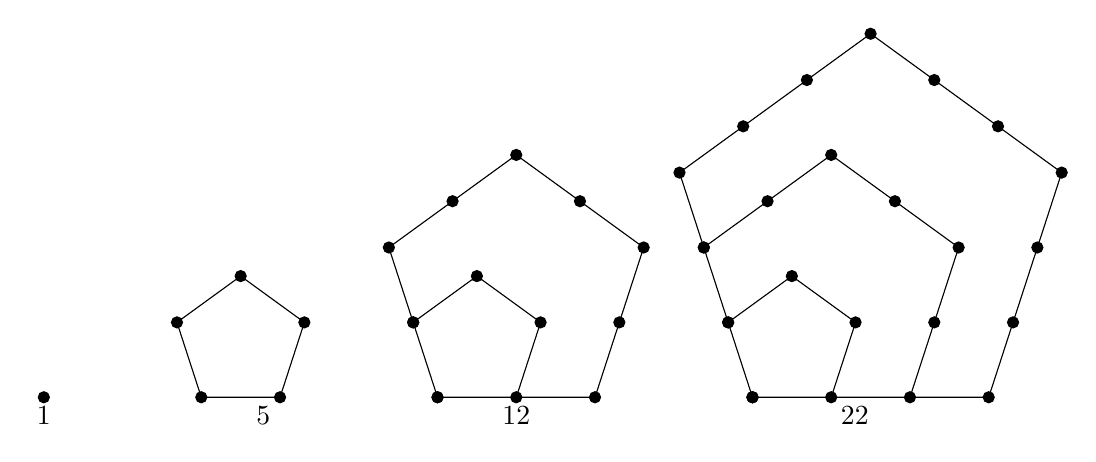
\begin{tikzpicture}
        \filldraw (0,0) node[below]{$1$} circle [radius=2pt];
        \filldraw (2,0) circle [radius=2pt] --++ (0:1)node[below left]{$5$} circle [radius=2pt] --++ (72:1) circle [radius=2pt] --++ (144:1) circle [radius=2pt] --++ (216:1) circle [radius=2pt] --++ (288:1) circle [radius=2pt];
        \filldraw (5,0) circle [radius=2pt] --++ (0:1) circle [radius=2pt] --++ (72:1) circle [radius=2pt] --++ (144:1) circle [radius=2pt] --++ (216:1) circle [radius=2pt] --++ (288:1) circle [radius=2pt];
        \filldraw (5,0) circle [radius=2pt] ++ (0:1)node[below]{$12$} --++ (0:1) circle [radius=2pt] --++ (72:1) circle [radius=2pt] --++ (72:1) circle [radius=2pt] --++ (144:1) circle [radius=2pt] --++ (144:1) circle [radius=2pt] --++ (216:1) circle [radius=2pt] --++ (216:1) circle [radius=2pt] --++ (288:1) circle [radius=2pt];
        \filldraw (9,0) circle [radius=2pt] --++ (0:1) circle [radius=2pt] --++ (72:1) circle [radius=2pt] --++ (144:1) circle [radius=2pt] --++ (216:1) circle [radius=2pt] --++ (288:1) circle [radius=2pt];
        \filldraw (9,0) circle [radius=2pt] ++ (0:1)node[below right]{$22$} --++ (0:1) circle [radius=2pt] --++ (72:1) circle [radius=2pt] --++ (72:1) circle [radius=2pt] --++ (144:1) circle [radius=2pt] --++ (144:1) circle [radius=2pt] --++ (216:1) circle [radius=2pt] --++ (216:1) circle [radius=2pt] --++ (288:1) circle [radius=2pt];
        \filldraw (9,0) circle [radius=2pt] ++ (0:2) --++ (0:1) circle [radius=2pt] --++ (72:1) circle [radius=2pt] --++ (72:1) circle [radius=2pt] --++ (72:1) circle [radius=2pt] --++ (144:1) circle [radius=2pt] --++ (144:1) circle [radius=2pt] --++ (144:1) circle [radius=2pt] --++ (216:1) circle [radius=2pt] --++ (216:1) circle [radius=2pt] --++ (216:1) circle [radius=2pt] --++ (288:1) circle [radius=2pt];
      \end{tikzpicture} 
\end{figure}
\item[Answer:] 1, 5, 12, 22, 35, 51, 70, $\ldots$
\begin{equation*}
  \text{here } a_n = \flatfrac{(3n^2 - n)}{2}
\end{equation*}
Hexagonal Numbers: 1, 6, 15, 28, 45, 66, 91, $\ldots$ , $2n^2 - n$, $\ldots$\\
Heptagonal Numbers:  1, 7, 18, 34, 55, 81, 112, $\ldots$, $\flatfrac{(5n^2 - 3n)}{2}$, $\ldots$
\end{enumerate}
\end{document}
